\documentclass[11pt]{article}
\usepackage[margin=2.3cm]{geometry}
\usepackage{amsmath,amssymb}
\usepackage{booktabs,tabularx}
\usepackage{graphicx}
\usepackage{enumitem}
\usepackage[dvipsnames]{xcolor}
\usepackage[most]{tcolorbox}
\usepackage{xurl}
\usepackage[colorlinks=true,linkcolor=MidnightBlue,urlcolor=MidnightBlue]{hyperref}
\setlist{itemsep=2pt,topsep=3pt}
\setlength{\parskip}{5pt}\setlength{\parindent}{0pt}
\newtcolorbox{lesson}{colback=green!4,colframe=green!45!black,title=Lesson,fonttitle=\bfseries\small,boxrule=0.6pt,arc=2pt}
\newtcolorbox{try}{colback=blue!3,colframe=blue!50!black,title=Try it,fonttitle=\bfseries\small,boxrule=0.6pt,arc=2pt}
\newtcolorbox{ours}{colback=orange!5,colframe=orange!70!black,title=What this means for our ROM,fonttitle=\bfseries\small,boxrule=0.6pt,arc=2pt}

\title{\textbf{Quadrature, step by step}\\[3pt]\large A study guide to the rules in Hari's off-mesh study:\\Gauss, lattice (Fibonacci/CBC), Sobol, Smolyak and Monte Carlo}
\author{Tunable-NM-ROM project}
\date{2026-10-07}

\begin{document}
\maketitle

\begin{tcolorbox}[colback=gray!4,colframe=gray!50,boxrule=0.5pt,arc=2pt]
\small\textbf{How to use this guide.} Read the steps in order; each takes a few minutes. Every number and figure is
produced by \texttt{exercises.py} in this folder (run it with
\texttt{/home/tahmid/Dev/.venv/bin/python exercises.py}), using an unchanged copy of Hari's rule code.
The 2D test integrand is an \emph{illustrative} smooth bump that behaves like ours; our real bank is
harder (it needs more points), so the absolute numbers here are not our paper's numbers.
\end{tcolorbox}

\tableofcontents

\section*{Step 0. The one problem every rule solves}
\addcontentsline{toc}{section}{Step 0. The one problem every rule solves}
Every time step, our reduced model needs, for each sine test function $\psi_{ab}(x,y)=\sin(a\pi x)\sin(b\pi y)$,
\[
N_{ab}=\int_0^1\!\!\int_0^1 f(x,y)\,dx\,dy,\qquad f=\psi_{ab}\;u\;(u_x+u_y),\qquad u(x,y)=G(x,y)\,c .
\]
We cannot integrate exactly, so we pick $m$ points $x_q$ and weights $w_q$ and use
\[
\int f\;\approx\;\sum_{q=1}^{m} w_q\,f(x_q).
\]
\textbf{That is all a quadrature rule is}: a list of points and weights. The rules below differ only in
\emph{where} the points go and \emph{how} they are weighted. Three facts about our integrand decide which rule wins:
\begin{enumerate}
\item it is very \textbf{smooth} (the bank is an analytic neural network);
\item it \textbf{vanishes at the walls} (the field is zero on the boundary, and so is each sine test);
\item it \textbf{oscillates}, because the tests go up to frequencies $a,b$ of roughly 25--45.
\end{enumerate}

\section*{Step 1. Three ways to integrate in 1D}
\addcontentsline{toc}{section}{Step 1. Three ways to integrate in 1D}
\begin{itemize}
\item \textbf{Equal spacing} (midpoint rule): $x_k=(k+\tfrac12)/n$, all weights $1/n$. This is the 1D version of a lattice.
\item \textbf{Monte Carlo}: $n$ random points, weights $1/n$.
\item \textbf{Gauss--Legendre}: $p$ special points (the roots of the Legendre polynomial $P_p$) with special weights.
It is the unique $p$-point rule that is \emph{exact for every polynomial of degree up to $2p-1$}.
\end{itemize}

\textbf{Check Gauss's promise.} A degree-5 polynomial needs $2p-1\ge5$, i.e.\ $p=3$:

\begin{center}\begin{tabular}{lr}
\toprule
Gauss points $p$ & error on a degree-5 polynomial \\
\midrule
1 & $7.0\times10^{-1}$ \\
2 & $9.7\times10^{-2}$ \\
3 & $2.2\times10^{-16}$ \\
4 & $8.9\times10^{-16}$ \\
\bottomrule
\end{tabular}
\end{center}

At $p=3$ the error drops to rounding level, exactly as promised.

\begin{center}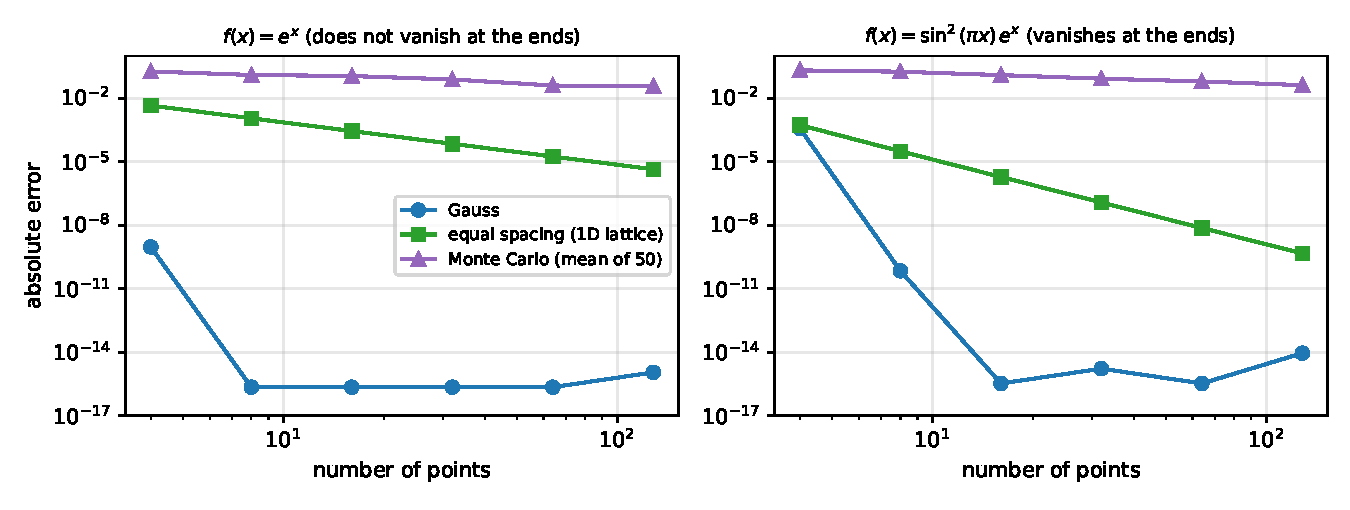
\includegraphics[width=\linewidth]{figs/s1_1d.pdf}\end{center}

\textbf{Look at the right panel.} When the integrand vanishes at both ends, equal spacing suddenly becomes much better.
Doubling the points cuts the error by:

\begin{center}\begin{tabular}{lrrr}
\toprule
integrand & error, 32 pts & error, 64 pts & ratio \\
\midrule
$e^x$ & $7.0\times10^{-5}$ & $1.7\times10^{-5}$ & 4.0 \\
$\sin^2(\pi x)e^x$ & $1.2\times10^{-7}$ & $7.4\times10^{-9}$ & 16.0 \\
\bottomrule
\end{tabular}
\end{center}

A ratio of 4 means error $\propto h^2$; a ratio of 16 means error $\propto h^4$. Vanishing at the ends removes the
``seam'' when the function is wrapped around periodically, and equal spacing is excellent for periodic functions.

\begin{lesson}
\begin{itemize}
\item Gauss is the champion for smooth functions: its error falls \emph{geometrically} (a straight line on a log plot).
\item Equal spacing is mediocre in general, but becomes very good when the integrand vanishes at the ends.
\item Monte Carlo is slow everywhere: its error falls only like $1/\sqrt n$.
\end{itemize}
\end{lesson}

\section*{Step 2. Oscillation: Gauss must first ``see'' the wiggles}
\addcontentsline{toc}{section}{Step 2. Oscillation: Gauss must first ``see'' the wiggles}
Multiply a smooth bump by $\sin(a\pi x)$ and integrate with Gauss:

\begin{center}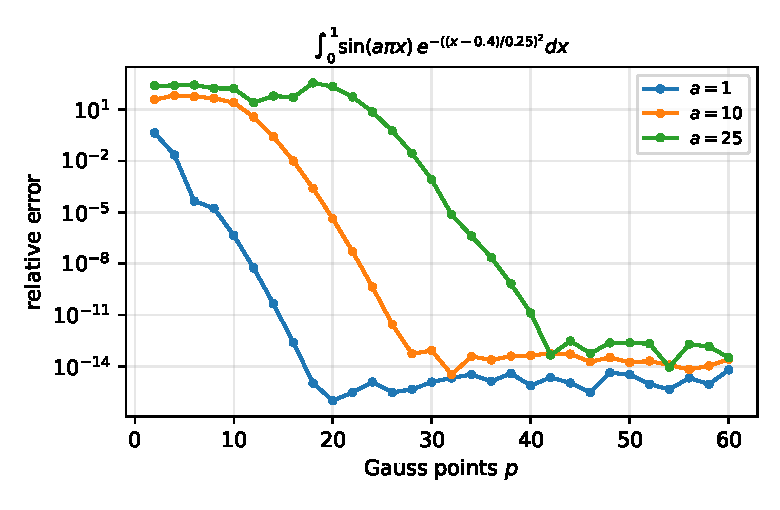
\includegraphics[width=0.62\linewidth]{figs/s2_oscillation.pdf}\end{center}
\begin{center}\begin{tabular}{lr}
\toprule
test frequency $a$ & first $p$ with error $<10^{-6}$ \\
\midrule
1 & 10 \\
10 & 22 \\
25 & 34 \\
\bottomrule
\end{tabular}
\end{center}

Nothing happens until $p$ is large enough to resolve the oscillation (roughly $p\gtrsim a$); after that the error
collapses geometrically.

\begin{ours}
Our tests go up to $a,b\approx25$--$45$, so a Gauss rule needs at least that many points \emph{per direction} before
it starts working. In 3D that is $p^3$ points, which is why Gauss $16^3$ failed on our 3D model and $24^3$--$32^3$ worked.
\end{ours}

\section*{Step 3. Going to 2D: five ways to place points}
\addcontentsline{toc}{section}{Step 3. Going to 2D: five ways to place points}
\begin{center}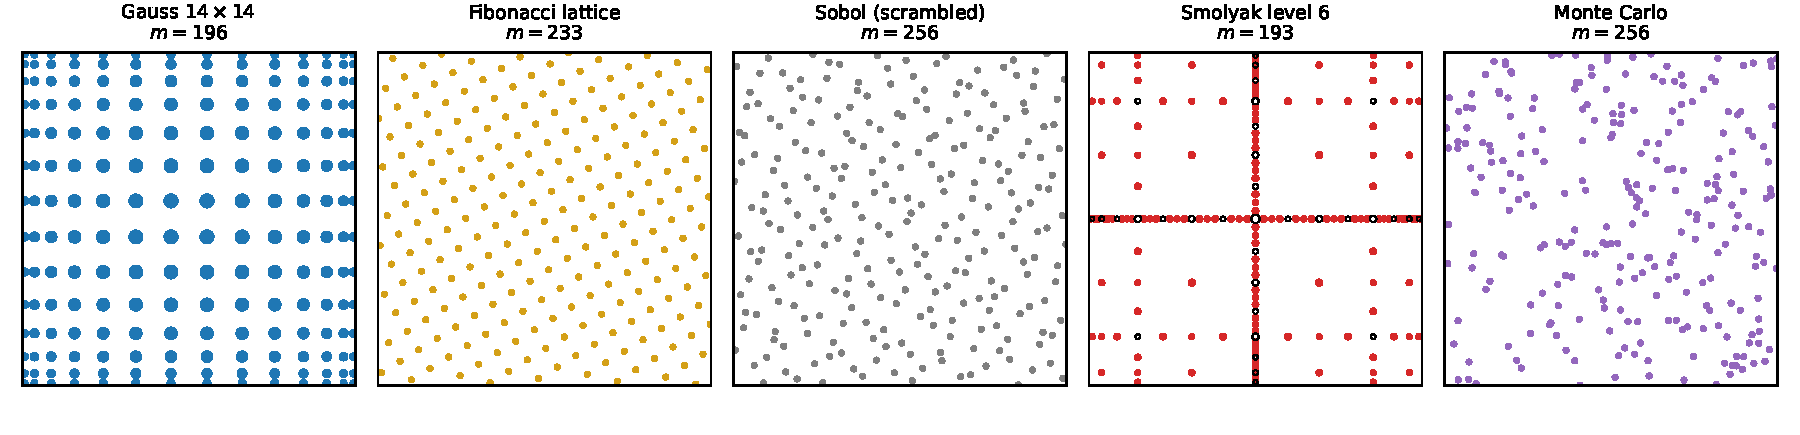
\includegraphics[width=\linewidth]{figs/s3_points.pdf}\end{center}
(Dot size shows the weight; open black circles in Smolyak are \emph{negative} weights.)

\subsection*{3a. Tensor Gauss}
Take the 1D Gauss rule in each direction and form all pairs: $x_q=(x_i,x_j)$, $w_q=w_iw_j$. That gives $p^2$ points in 2D
and $p^3$ in 3D. It inherits Gauss's geometric convergence, but the point count is cubed in 3D.

\subsection*{3b. Rank-1 lattice (Fibonacci in 2D, CBC in 3D)}
Choose an integer vector $z$ and a random shift $\Delta$, and use equal weights:
\[
x_k=\Big\{\tfrac{k\,z}{m}+\Delta\Big\},\qquad w_k=\tfrac1m,\qquad k=0,\dots,m-1,
\]
where $\{\cdot\}$ keeps the fractional part (wraps around the square). The points form a tilted, perfectly even grid.
\begin{itemize}
\item \textbf{Fibonacci (2D):} $m=F_k$ (a Fibonacci number) and $z=(1,F_{k-1})$, for example $m=233$, $z=(1,144)$.
This is the best possible lattice in 2D.
\item \textbf{CBC (3D and higher):} ``component by component''. Pick $z_1=1$, then choose $z_2$ to minimise an error
measure, then $z_3$ given $z_1,z_2$, and so on. It is cheap to build and close to optimal in any dimension.
\end{itemize}

\subsection*{3c. Sobol (quasi-Monte Carlo)}
A deterministic sequence built from binary digits so that every small box of the square receives its fair share of points
(``low discrepancy''). Weights are $1/m$. ``Scrambled'' means the digits are randomly permuted, which keeps the evenness
and makes the error estimate unbiased.

\subsection*{3d. Smolyak sparse grid}
Instead of the full $p\times p$ tensor grid, add up \emph{small} tensor grids of 1D rules at different resolutions, with
plus and minus signs:
\[
A(q,d)=\sum_{q-d+1\le|\mathbf i|\le q}(-1)^{q-|\mathbf i|}\binom{d-1}{q-|\mathbf i|}\,Q_{i_1}\otimes\cdots\otimes Q_{i_d}.
\]
Fine resolution along one axis is only ever combined with coarse resolution along the other, so the points form a cross.
It needs far fewer points than $p^d$, but some weights are negative.

\subsection*{3e. Monte Carlo}
Random points, weights $1/m$. It is the baseline that every other rule should beat.

\section*{Step 4. The race on an integrand like ours}
\addcontentsline{toc}{section}{Step 4. The race on an integrand like ours}
Integrand: $f=\psi_{ab}\,u\,(u_x+u_y)$ with a smooth bump $u$ that vanishes on the walls. Error is divided by $\int|f|$
(the size of the integrand). Two test functions: a gentle one, $\psi_{3,4}$, and a mixed high-frequency one, $\psi_{12,12}$.

\begin{center}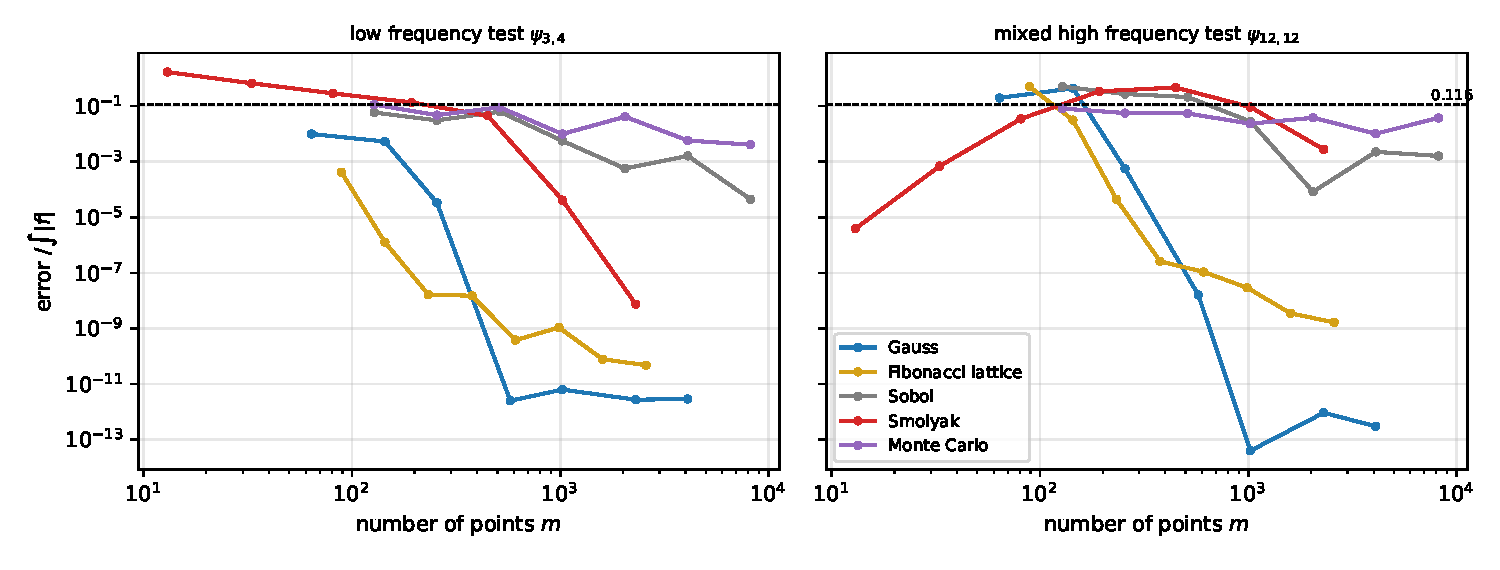
\includegraphics[width=\linewidth]{figs/s4_convergence.pdf}\end{center}
\begin{center}\small\begin{tabular}{lrrrr}
\toprule
rule & $m$ & error, $\psi_{3,4}$ & $m$ & error, $\psi_{12,12}$ \\
\midrule
Gauss & 4096 & $2.9\times10^{-12}$ & 4096 & $3.0\times10^{-13}$ \\
Fibonacci lattice & 2584 & $4.8\times10^{-11}$ & 2584 & $1.7\times10^{-9}$ \\
Sobol & 4096 & $1.6\times10^{-3}$ & 4096 & $2.2\times10^{-3}$ \\
Smolyak & 2305 & $7.5\times10^{-9}$ & 2305 & $2.7\times10^{-3}$ \\
Monte Carlo & 4096 & $5.8\times10^{-3}$ & 4096 & $1.0\times10^{-2}$ \\
\bottomrule
\end{tabular}
\end{center}

\begin{lesson}
\begin{itemize}
\item \textbf{Gauss and the lattice are orders of magnitude ahead.} Both exploit smoothness.
\item \textbf{Sobol and Monte Carlo plateau.} They don't exploit smoothness at all.
\item \textbf{Smolyak is fine on the gentle test and far worse on $\psi_{12,12}$.} A sparse grid only keeps
``high detail in one direction at a time''. A test that is high-frequency in \emph{both} directions is exactly what it throws away.
\end{itemize}
\end{lesson}

\section*{Step 5. Why the lattice works: aliasing}
\addcontentsline{toc}{section}{Step 5. Why the lattice works: aliasing}
Write $f$ as a Fourier series $f(x)=\sum_h \hat f(h)e^{2\pi i h\cdot x}$. A lattice sum gets every frequency exactly right
\emph{except} those it cannot tell apart from zero, the ``dual lattice'' $h\cdot z\equiv0 \pmod m$:
\[
\frac1m\sum_k f(x_k)-\int f=\sum_{\substack{h\ne0\\ h\cdot z\equiv 0\ (\mathrm{mod}\ m)}}\hat f(h)\,e^{2\pi i h\cdot\Delta}.
\]
\begin{itemize}
\item A good $z$ (Fibonacci or CBC) pushes those aliased frequencies out to very high $h$.
\item A smooth integrand has tiny Fourier coefficients there, so the error is tiny.
\item Vanishing at the walls makes the wrapped-around function nearly seamless, so its coefficients decay fast (Step 1 again).
\item The remaining kink at the walls sets an \emph{algebraic} rate, not Gauss's geometric one. But that rate does not get
worse with dimension, whereas Gauss needs $p^d$ points. \textbf{That is why lattices beat Gauss in 3D.}
\end{itemize}

\textbf{Random shift.} The shift $\Delta$ changes the error a little. Repeating with 32 random shifts gives a spread,
which serves as a free error indicator:
\begin{center}\begin{tabular}{lrr}
\toprule
lattice points $m$ & median over 32 shifts & worst over 32 shifts \\
\midrule
233 & $1.4\times10^{-7}$ & $3.2\times10^{-7}$ \\
610 & $6.3\times10^{-9}$ & $1.6\times10^{-8}$ \\
1597 & $4.6\times10^{-10}$ & $1.0\times10^{-9}$ \\
\bottomrule
\end{tabular}
\end{center}

\section*{Step 6. The tent transform (and why it does not help here)}
\addcontentsline{toc}{section}{Step 6. The tent transform (and why it does not help here)}
Lattices are designed for periodic functions. The textbook fix for a non-periodic integrand is the ``tent'' map
$x\mapsto 1-|2x-1|$, which folds the square so that the function becomes periodic. Our integrand already vanishes at the
walls, so it is nearly periodic anyway, and the tent only doubles the frequencies the rule has to resolve:
\begin{center}\begin{tabular}{lrr}
\toprule
$m$ & plain lattice & with tent transform \\
\midrule
233 & $6.9\times10^{-8}$ & $1.1\times10^{-1}$ \\
610 & $5.5\times10^{-9}$ & $6.2\times10^{-7}$ \\
1597 & $2.8\times10^{-10}$ & $2.7\times10^{-9}$ \\
\bottomrule
\end{tabular}
\end{center}

\begin{ours}
Hari observed the same: tent always hurt. His explanation (``it adds a kink'') turns out to be wrong for this
integrand. The tent actually makes it smoother; the loss comes from the doubled frequencies. This is one of the
corrections the paper will carry.
\end{ours}

\section*{Step 7. The twist: the mesh's answer is not the true answer}
\addcontentsline{toc}{section}{Step 7. The twist: the mesh's answer is not the true answer}
The full-order solver does not compute $\int f$. It computes a \textbf{mesh sum} with a first-order upwind difference
for $u_x,u_y$:
\[
h^2\sum_{\text{nodes } i}\psi_{ab}(x_i)\,u_i\,(D^{\mathrm{up}}u)_i,\qquad D^{\mathrm{up}}u\approx u_x+u_y+O(h).
\]
Compare it with the true integral as the mesh is refined:
\begin{center}\begin{tabular}{lrr}
\toprule
mesh $N$ & mesh sum vs true integral & ratio to previous \\
\midrule
32 & $7.5\times10^{-1}$ & -- \\
64 & $3.8\times10^{-1}$ & 1.96 \\
128 & $1.9\times10^{-1}$ & 1.98 \\
256 & $9.6\times10^{-2}$ & 1.99 \\
512 & $4.8\times10^{-2}$ & 2.00 \\
\bottomrule
\end{tabular}
\\[4pt]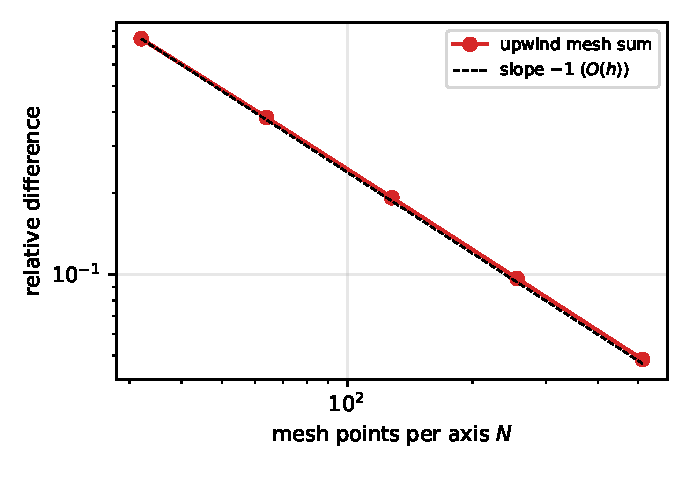
\includegraphics[width=0.5\linewidth]{figs/s7_gap.pdf}\end{center}

The gap halves with every doubling of the mesh: it is an $O(h)$ discretisation error.
\begin{itemize}
\item The \textbf{old methods} (mesh sub-lattice, fitted EQ, precomputed tensor) all reproduce the mesh sum, gap included.
\item An \textbf{off-mesh rule} integrates the true $\int f$ using the bank's exact gradient, so the gap never enters.
\end{itemize}

\begin{ours}
This is why, on the 3D model, the old tensor's error shrank with the mesh while the off-mesh error stayed the same at
every mesh. It is also why the paper needs better (second-order) references: part of the measured gain may simply be
that the first-order mesh sum is crude.
\end{ours}

\section*{Step 8. Putting it into the reduced model}
\addcontentsline{toc}{section}{Step 8. Putting it into the reduced model}
\begin{enumerate}
\item \textbf{Offline, once:} decode the bank and its gradient at the $m$ rule points: $B=G(x_q)$ and $D=\partial G(x_q)$,
each $m\times R'$.
\item \textbf{Online, every iteration:} $u(x_q)=Bc$ and $(u_x+u_y)(x_q)=Dc$; multiply pointwise, then weight by
$w_q\psi_{ab}(x_q)$ and sum: $N(c)=P^\top[(Bc)\odot(Dc)]$.
\item \textbf{Cost} depends on $m$, $R'$ and $M$ only, not on the mesh. \textbf{Storage} is $m(2R'+M)$ numbers, against
$MR'^2$ for the precomputed tensor.
\item \textbf{No fitting:} the points are a formula, the same for every mesh and every dataset.
\end{enumerate}

\section*{Cheat sheet}
\addcontentsline{toc}{section}{Cheat sheet}
\small
\begin{tabularx}{\linewidth}{@{}l X X X l@{}}
\toprule
rule & points & weights & how the error falls (smooth integrand) & role in our study\\
\midrule
Gauss (tensor) & $p^d$, Legendre roots & Gauss weights & geometrically, once $p$ resolves the tests & best in 2D\\
Lattice (Fibonacci/CBC) & $m$ on a tilted even grid & $1/m$ & algebraically (fast if the integrand vanishes at the walls); does not degrade with dimension & best in 3D\\
Sobol & $m$, base-2 low-discrepancy & $1/m$ & about $1/m$ & control\\
Smolyak & sparse cross & mixed signs & fine for gentle tests; fails on mixed high frequencies & must-fail control\\
Monte Carlo & $m$ random & $1/m$ & $1/\sqrt m$ & baseline\\
\bottomrule
\end{tabularx}
\normalsize

\section*{Check yourself}
\addcontentsline{toc}{section}{Check yourself}
\begin{enumerate}
\item Why does 3-point Gauss integrate $x^5$ exactly but not $x^6$? \emph{(Exact up to degree $2p-1=5$.)}
\item Why does equal spacing get so much better when the integrand vanishes at the ends? \emph{(The periodic wrap has no
seam, so the Fourier coefficients decay fast.)}
\item Why is Gauss $16^3$ useless for our 3D model? \emph{(16 points per direction cannot resolve test frequencies of 25+.)}
\item Why do lattices beat Gauss in 3D but not in 2D? \emph{(Gauss pays $p^d$; the lattice's rate does not degrade with $d$.)}
\item Why does Smolyak fail on $\psi_{12,12}$ but not on $\psi_{3,4}$? \emph{(It discards detail that is high in both directions at once.)}
\item Why can an off-mesh rule be \emph{more} accurate than the full solver's own mesh sum? \emph{(The mesh sum has an
$O(h)$ upwind error; the off-mesh rule targets the true integral.)}
\item What still grows with the mesh in an off-mesh ROM? \emph{(Projecting the initial field and decoding the output on the mesh.)}
\end{enumerate}

\section*{Glossary}
\addcontentsline{toc}{section}{Glossary}
\small
\begin{description}[leftmargin=0pt]
\item[quadrature rule] points $x_q$ and weights $w_q$ approximating an integral by $\sum w_q f(x_q)$.
\item[$m$, $p$] number of points; points per direction for a tensor rule ($m=p^d$).
\item[geometric / algebraic convergence] error $\sim \varrho^{-p}$ (straight line on a log plot) vs error $\sim m^{-k}$ (straight line on a log--log plot).
\item[test function $\psi_{ab}$] the sine $\sin(a\pi x)\sin(b\pi y)$ against which the equation is checked.
\item[dual lattice / aliasing] the frequencies a lattice cannot distinguish from zero; they make up its entire error.
\item[random shift] moving the whole lattice by a random offset; the spread over shifts estimates the error.
\item[low discrepancy] points that fill every sub-box evenly (Sobol).
\item[sparse grid] a combination of small tensor grids (Smolyak).
\item[upwind difference] a one-sided derivative taken from the side the flow comes from; first-order accurate.
\item[$O(h)$ gap] the difference between the mesh sum and the true integral; halves when the mesh is refined.
\item[bank $G$, $R'$, $M$] the network basis, the number of basis functions used, the number of test functions.
\item[off-mesh] evaluating the bank at rule points that are not mesh nodes.
\end{description}

\end{document}
